\newcommand{\phiR} {\ensuremath{\phi\sups{\textsc{r}}}\xspace}
\newcommand{\phiI} {\ensuremath{\phi\sups{\textsc{i}}}\xspace}
\newcommand{\phiRd}{\ensuremath{    \pdiff{\phiR}{\delta}   }\xspace}
\newcommand{\phiId}{\ensuremath{    \pdiff{\phiI}{\delta}   }\xspace}
\newcommand{\phiRt}{\ensuremath{    \pdiff{\phiR}{\tau  }   }\xspace}
\newcommand{\phiIt}{\ensuremath{    \pdiff{\phiI}{\tau  }   }\xspace}
\newcommand{\phid}{\ensuremath{     \pdiff{\phi} {\delta}   }\xspace}
\newcommand{\phit}{\ensuremath{     \pdiff{\phi} {\tau  }   }\xspace}
\newcommand{\Helm} {\ensuremath{\phi (\delta,\tau)}\xspace}
\newcommand{\HelmI}{\ensuremath{\phiI(\delta,\tau)}\xspace}
\newcommand{\HelmR}{\ensuremath{\phiR(\delta,\tau)}\xspace}



\appendix{Thermophysical Properties}\label[appendix]{Appendix:THProperties}

\section{Equation of State}\label{Section:EOS}

The \EOS used for the simulations is the \Acronym{IAPWS} Formulation 1995 for the Thermodynamic Properties of Ordinary Water Substance for General and Scientific Use (IAPWS-95) \cite{iapws_revised_2009}.
The specifics of the \EOS are discussed in the following section.
Also, the procedure for back-calculating the temperature given a density and internal energy from the formulation is outlined since the conservation laws for the simulations evolve the internal energy based on mechanical balance but the \EOS uses temperature for explicit calculation of state properties.

\subsection{IAPWS Formulation 1995}
The IAPWS-95 is a fully non-ideal \EOS for water that uses on an empirical curve fit of the Helmholtz Free Energy potential \Afe.
The natural variables of the potential are density \Density and temperature \Temperature, and the formulation uses a dimensionless density \delta and a dimensionless temperature \tau defined by 
\begin{align}
    \delta &= \frac{\rho}{\rhoc} \Skip
    \tau   &= \frac{\Tc}{T}
\end{align}
where \rhoc and \Tc are, respectively, the critical point density and temperature of water.
The dimensionless form of the potential is the fundamental basis of the \Acronym{IAPWS} formulation and has the form
\begin{equation}
    \frac{\Afe(\rho,T)}{R\,T} = \Helm = \HelmI + \HelmR,
\end{equation}
where \phiI is an ideal gas potential function, \phiR is a residual (i.e., non-ideal gas) potential function, and $R$ is the specific gas constant of water.
The actual functional form of \Helm is cumbersome and will not be presented here (see \cite{iapws_revised_2009} for a full description).
Using this potential and its associated derivatives, all thermodynamic properties can be calculated for a given state.
A select group of relationships between the potential and properties are presented in \cref{Table:HFERelations}.
The relationships are valid for the entire set of single phase states.

\begin{table}[h!]
    \centering
    \newcommand{\Pull     }[1][-0.8em]{\hspace{#1}}
    \newcommand{\Push     }[1][ 0.5em]{\hspace{#1}}
    \newcommand{\EqualSign}[1][-0.8em]{\Pull[#1]$=$}
    \caption{Select thermodynamic properties and associated dimensionless \HFE relationships.}
    \label{Table:HFERelations}
    \rowcolors{2}{}{Gray}
    \begin{tabular}{c c c l}
        \toprule
        Property  & \multicolumn{3}{c}{Helmholtz Potential Relation} \\\midrule
        Pressure 
            &\Push$\dfrac{P}{R\rhoc\Tc} $&\EqualSign&\Pull$  \left[1 + \delta \phiRd\right]\dfrac{\delta}{\tau}$ \TableSkip
        Internal Energy
            &\Push$\dfrac{i}{R\,\Tc}    $&\EqualSign&\Pull$   \phit    $  \TableSkip
        Entropy
            &\Push$\dfrac{s}{R}         $&\EqualSign&\Pull$  \tau\phit - \phi$ \TableSkip
        Enthalpy
            &\Push$\dfrac{h}{R\Tc}      $&\EqualSign&\Pull$ \dfrac{1}{\tau}\left[1 + \tau \phit + \delta \phiRd\right]    $ \TableSkip
        \bottomrule
    \end{tabular}
\end{table}

Additionally, the formulation permits calculation of saturated properties.
Unlike the explicit, single phase equations above, saturated calculations involve a necessarily iterative procedure.
Solving for a saturated condition involves leveraging the three equilibrium conditions of phase change: constant pressure, constant temperature, and phasic equality of Gibbs free energy.  
In terms of the non-dimensional \HFE function \Helm, these equilibrium conditions form a system of equations that must be simultaneously satisfied:
\begin{subequations}\label{Eqn:TCS}
    \begin{align}
        \dfrac{\Psat}{R\rhoc\Tc} &= \left[1 + \deltaL \phiRd(\deltaL,\tauSat)\right]\dfrac{\deltaL}{\tauSat}    \label{Eqn:TCS:Pmatch1}\Skip
        \dfrac{\Psat}{R\rhoc\Tc} &= \left[1 + \deltaG \phiRd(\deltaG,\tauSat)\right]\dfrac{\deltaG}{\tauSat}    \label{Eqn:TCS:Pmatch2}\Skip
        \dfrac{\Psat}{R\rhoc\Tc} &= \left[\Ln\!\left(\frac{\deltaL}{\deltaG}\right) + 
                                          \phiR(\deltaL,\tauSat) - \phiR(\deltaG,\tauSat)\right] 
                                     \frac{\deltaL\deltaG}{\tauSat(\deltaL - \deltaG)}                          \label{Eqn:TCS:MaxwellCriterion}.
    \end{align}
\end{subequations}
\Cref{Eqn:TCS:Pmatch1,Eqn:TCS:Pmatch2} arise from the definition of pressure in terms of the \HFE and the pressure equality of the functions given the saturated liquid density \rhol and gas density \rhog at the saturation temperature.
\Cref{Eqn:TCS:MaxwellCriterion} is the Maxwell construction (i.e., equal area rule) of the Gibbs free energy equivalence (\cite{gould_chemical_2010}).  
The above system consists of three equations and four unknowns: \Psat, \tauSat, \deltaL, and \deltaG; therefore, the system can be solved once one of the saturation values is specified.
A pressure-volume diagram is shown in \cref{Fig:PvDiagram} calculated from an implementation of the IAPWS-95 formulation.

\begin{figure}%
    \begin{center}
        \caption{Pressure versus specific volume with several isotherms.  The gray line denotes the phase coexistence curve.}%
        \label{Fig:PvDiagram}%
        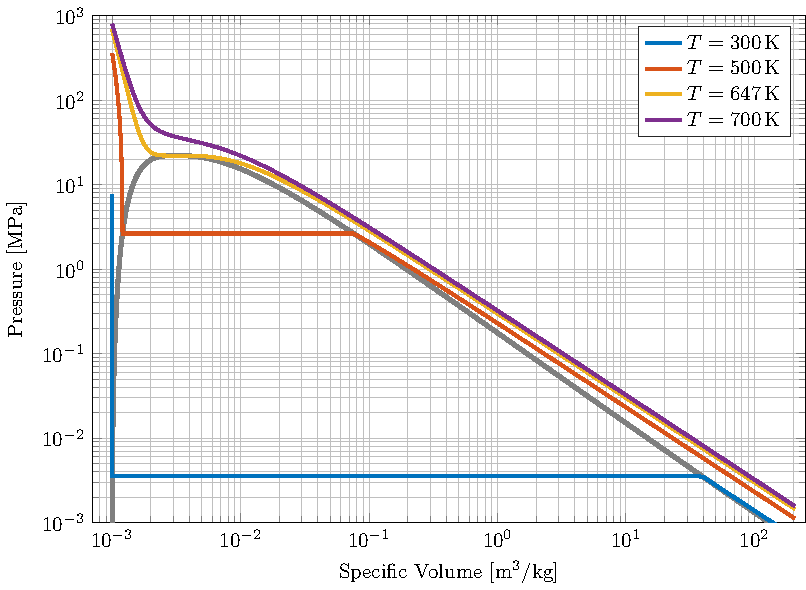
\includegraphics[scale=0.16]{PressureVsVolume}%7
    \end{center}
\end{figure}


\subsection{Back Calculation of Temperature}
Temperature is a very powerful state variable because it is a directly measurable quantity that provides a qualitative measurement of a fluid's internal energy.
However, in the balance equations \cref{Eqn:HEMBasic}, density and internal energy are the variables that are mechanically balanced, completely independent of thermodynamics. 
As such, it is most natural to update the thermodynamic and transport quantities with the mechanically specified density and internal energy to have a consistent evolution system.
Furthermore, since density and internal energy are defined and independent in the two-phase region (unlike pressure and temperature), the time evolution may lead to mixture quantities.

The solution procedure chosen relies on one key fact about the relationship between internal energy and temperature: 
along an arbitrary isochore, internal energy is an injective, monotonic function of temperature.
One result of this fact is that a single phase internal energy will always be higher than its saturation value at the current density; this allows for an explicit determination of one- or two-phase conditions (see \cref{Fig:IntERhoDiagram} for a phase diagram).
Another result is that root-finding procedures can be readily used to calculate the temperature for a state defined by density and internal energy.
In the single phase region with a given guess value, the dimensionless temperature is calculated by driving the following residual formula to zero through Newton's method:
\begin{equation}
    R(\tau) = \phit(\delta,\tau) - \frac{i}{R\Tc}.
    \label{Eqn:SinglePhaseResidualForTemperature}
\end{equation}
For the two-phase region, the situation is a bit more complicated since the mixture internal energy must be calculated at every temperature update and $\partial\phi/\partial\tau$ approximated numerically since no closed form exists.
The full algorithm is outlined below.
Once the temperature has been calculated, all other properties can be directly solved for using the natural variables of the Helmholtz potential.


\begin{BoxedAlgorithm}
    \DontPrintSemicolon
    \SetAlgoLined
    \SetKwInput{Input}{Input}
    \SetKwInput{Output}{Output}
    
    \begin{spacing}{1.1}
    % Algorithm begin
    \TitleOfAlgo{Temperature Back Calculation}
    \Input{A known dimensionless density \delta and internal energy \IntEnergy.}
    \Output{Corresponding dimensionless temperature \tau.}
    
    \vspace{0.5em}
    \isat = \mbox{GetSaturationInternalEnergy}(\delta)\;
    \eIf{ \IntEnergy $>$ \isat }{  
        \textsc{\% Single phase solve}\;
        $\tau  = \tau\subs{guess}$\;
        $d\tau = \Inf$\;
        \While{$\Abs(d\tau) > \varepsilon$}{
            $d\tau = - \Rez\subs[\!]{one}(\tau)/\Rez'\subs[\!\!\!]{one}(\tau)$\;
            $\tau = \tau + d\tau$\;
        }
    }{
        \textsc{\% Two-phase solve}\;
        $\tau  = \tau\subs{guess}$\;
        $d\tau = \Inf$\;
        \While{$\Abs(d\tau) > \varepsilon$}{
            $[\Psat,\deltaL,\deltaG] = \mbox{GetSaturationProperties}(\tau)$\;
            $ d\tau = - \Rez\subs[\!]{two}(\tau)/\Rez'\subs[\!\!\!]{two}(\tau)$\;
            $\tau = \tau + d\tau$\;
        }
    }
    \end{spacing}
\end{BoxedAlgorithm}
Above is an algorithmic outline of the temperature back calculation.  
The functions GetSaturationInternalEnergy() and GetSaturationProperties() rely on solving \cref{Eqn:TCS} 
through another Newton method.
The residual $\Rez\subs[\!]{one}$ is the same as \cref{Eqn:SinglePhaseResidualForTemperature} 
while $\Rez\subs[\!]{two}$ calculates the mixture internal energy at the current $\tau$ iterant 
and the approximates the derivative in the vapor dome (since there is no closed form).

\begin{figure}[H]%
    \begin{center}
        \caption[Internal energy versus density with an arbitrary isochore]{ 
                    Internal energy versus density with an arbitrary isochore.  
                    From the shape of the vapor dome in \Density-\IntEnergy space, it is clear that the saturation internal energy 
                    is always less than the single phase along an isochore.
        }%
        \label{Fig:IntERhoDiagram}%
        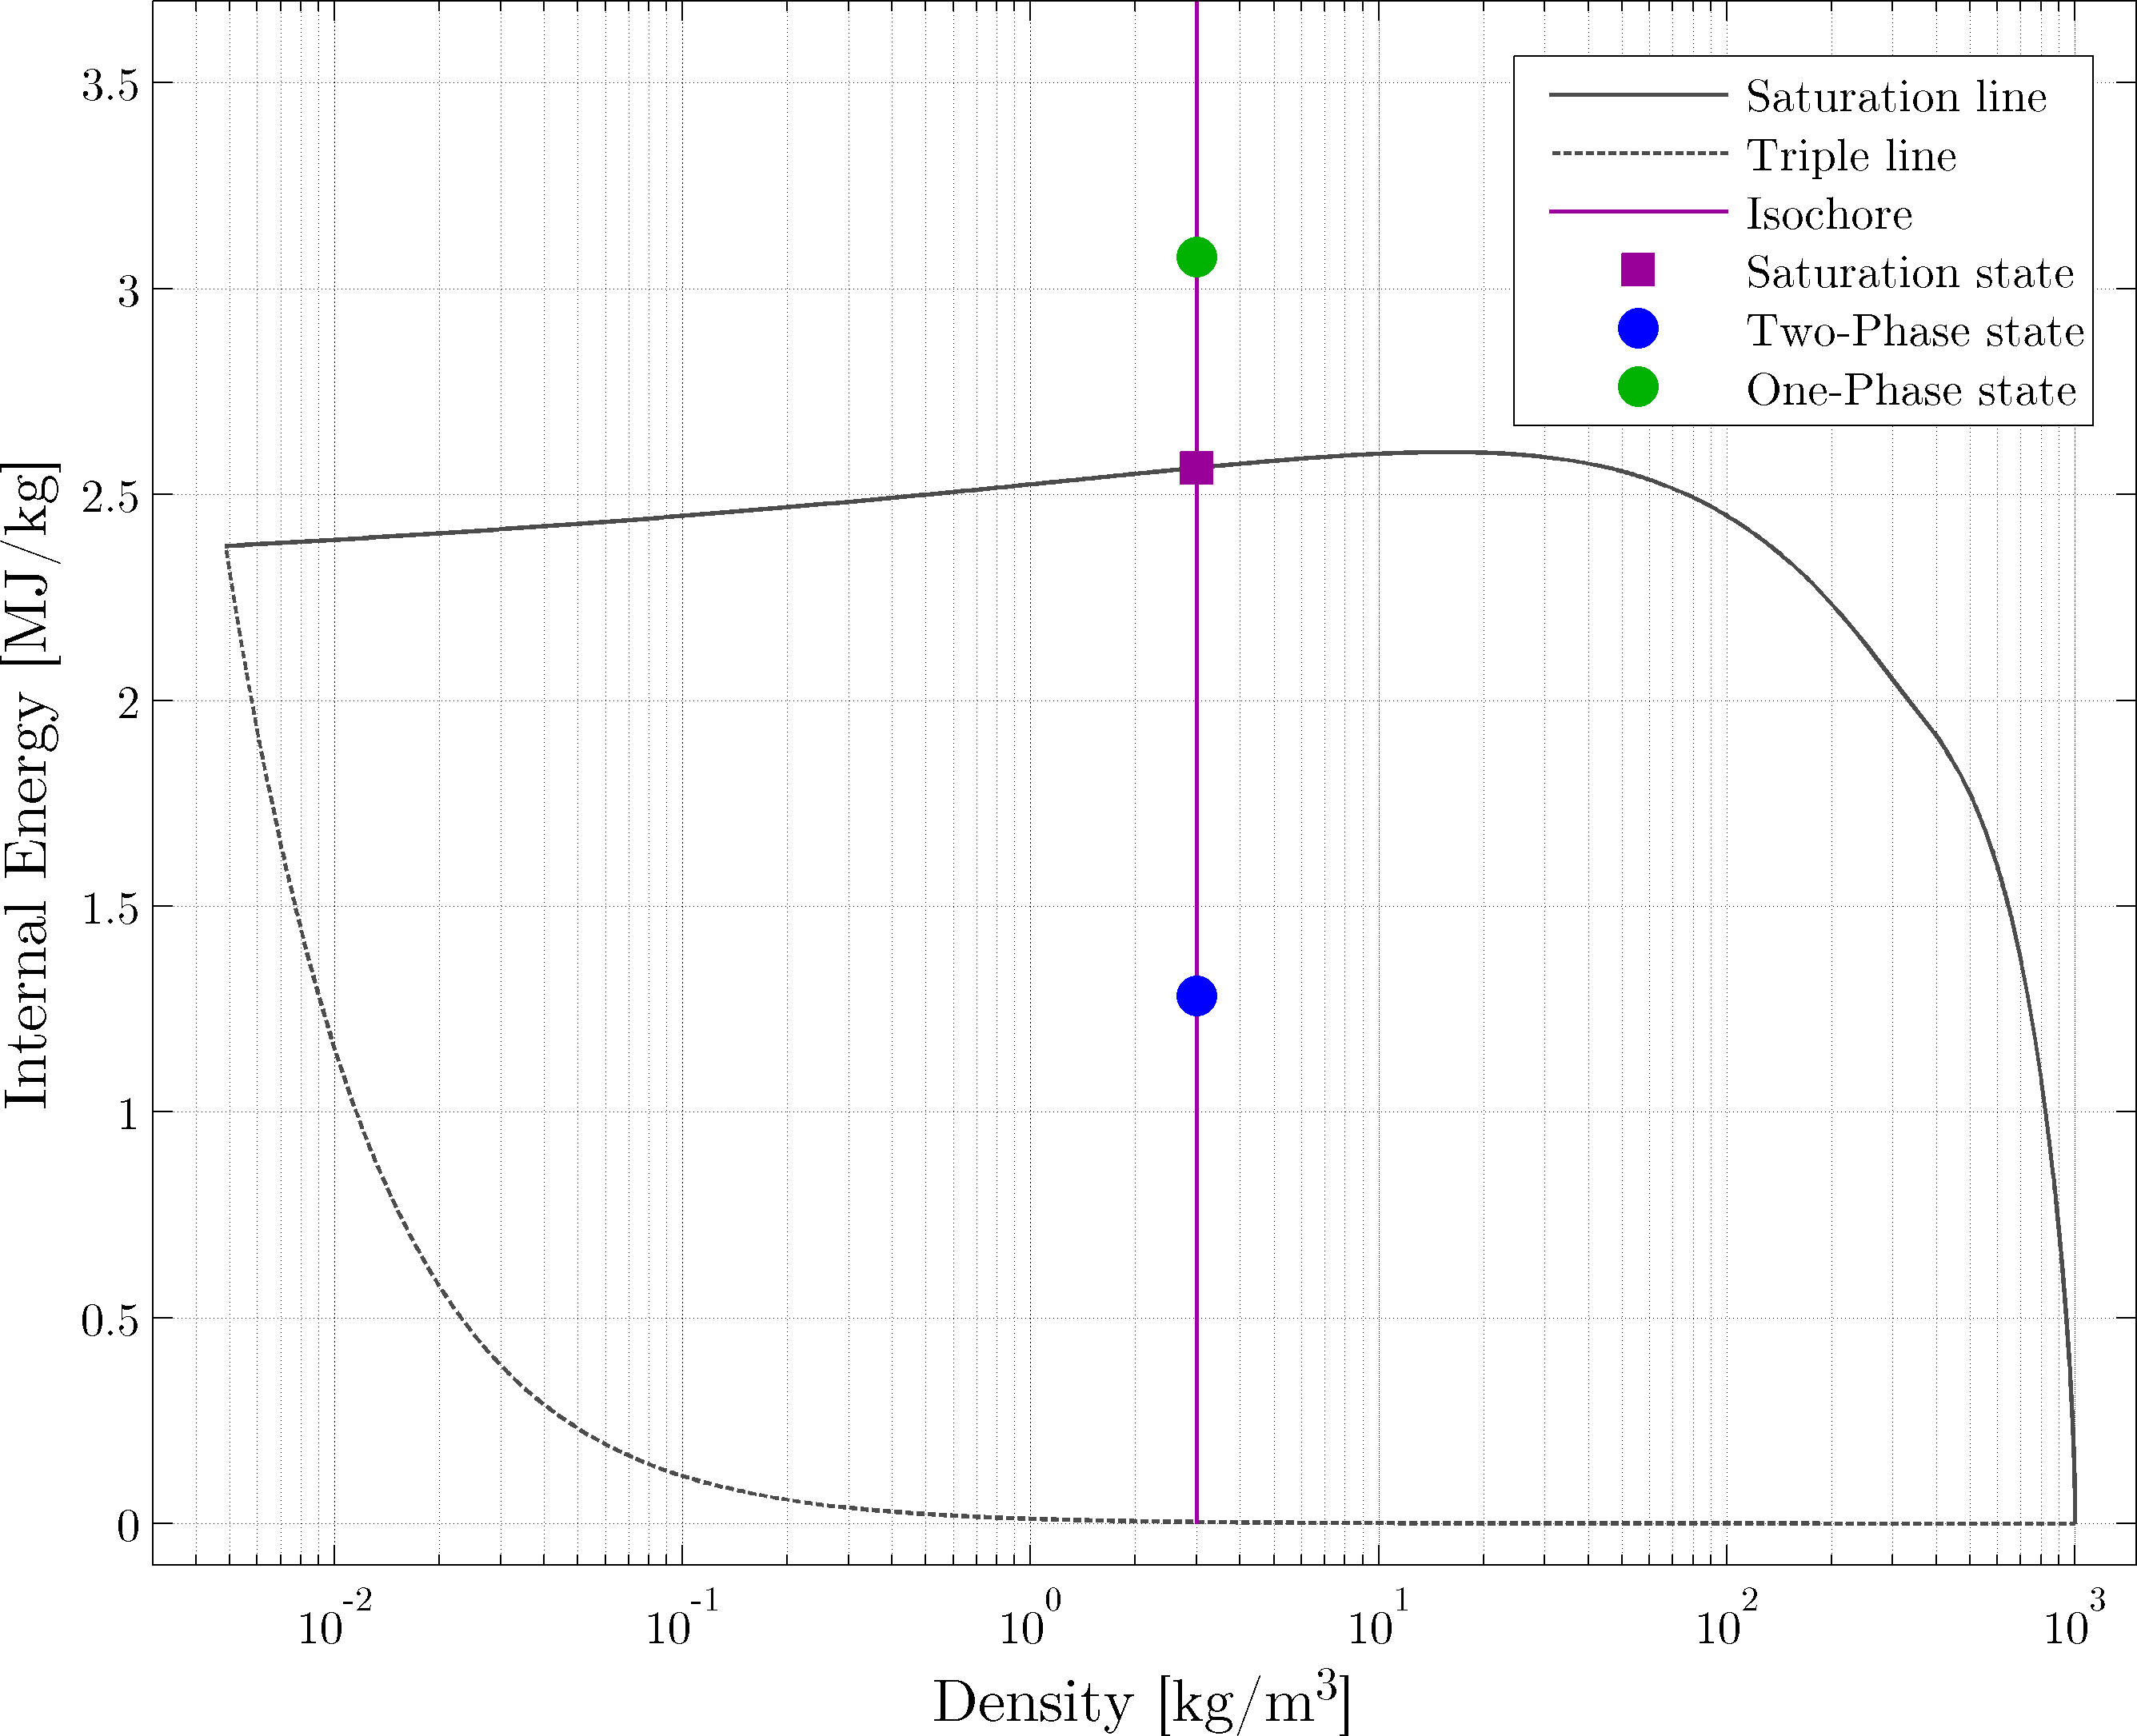
\includegraphics[scale=0.16]{InteEnergyVsDensity}%7
    \end{center}
\end{figure}

\cleardoublepage
\section{Transport Properties}\label{Section:TransportProps}
Thermal conductivity \ThCond and dynamic viscosity \Viscosity are transport properties and have no direct relation to thermodynamic potentials.
However, the \Acronym{IAPWS} has curve fits that are functions of density and temperature and are meant to be used in conjunction with the IAPWS-95 \EOS \cite{iapws_release_2008,iapws_release_2011}.


